\documentclass[12pt,letterpaper]{article}
\usepackage{pdfpages}
\usepackage{fancyhdr}
\usepackage[colorlinks=true, urlcolor=blue, linkcolor=blue]{hyperref}
\usepackage{graphicx}
\usepackage[top=1.4in, left=0.5in, right=0.5in, bottom=0.8in]{geometry}
\usepackage[T1]{fontenc}
\usepackage{helvet}
\pagestyle{fancy}
\renewcommand{\headrulewidth}{0pt}
\renewcommand{\footrulewidth}{0pt}
\setlength{\parindent}{0em}
\setlength{\parskip}{1em}


\fancyfoot[C]{\setlength{\unitlength}{1in}\begin{picture}(5,0)\put(-1.8,-1){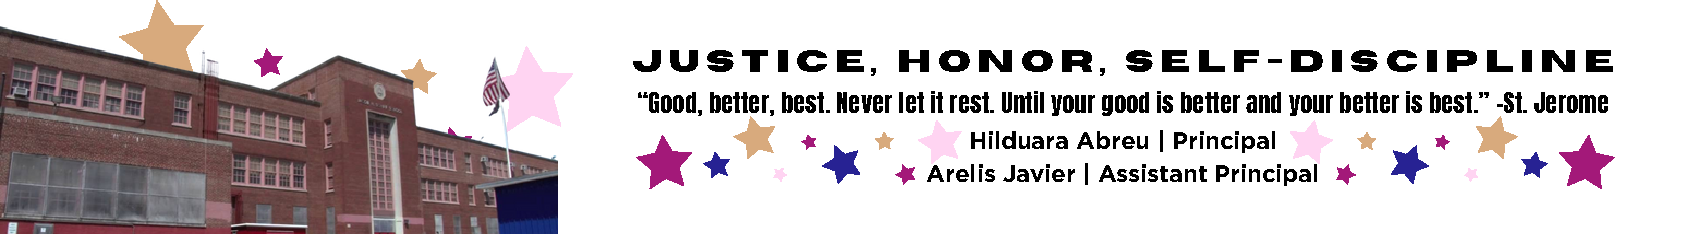
\includegraphics[width=8.8in,height=1.3in]{logo-1}}\end{picture}}
\fancyhead[C]{\setlength{\unitlength}{1in}\begin{picture}(5,0)\put(-1.9,-1){
\includegraphics[width=8.9in,height=1.3in]{logo-2}}\end{picture}}

\pagenumbering{gobble}
\addtolength{\evensidemargin}{-2in}
\addtolength{\topmargin}{-0.5in}
\addtolength{\textwidth}{0in}
%%%%%%%%%%%%%%%%%%%%%%%%%%%%%%%%%%%%%%%%%%%%%%%%%%%%%%%%%%%%%%%%%%

\begin{document}
\vspace*{0.5in}
Date: \href{https://www.ps192.org}{2024-25} 

\textbf{Subject: Welcome Letter 3-K and Pre-K}

Dear Families,

We're excitedly counting down the days until the arrival of our students on Thursday, September 5th, 2024! Our dedicated instructors and school staff are eagerly looking
forward to welcoming you to what promises to be a thrilling year of fostering connections
and building a strong community. Our caring educators are excited to share their laughter,
energy, and passion for learning with your children.

As we gear up for your child's return, we want to share important information in place at
P.S. 192 to ensure a safe and enjoyable learning experience for everyone. Please take note
of the following guidelines:
	\begin{itemize}
	\item Uniforms: All students are required to come to school daily dressed in their
	uniforms, which remain the same: a burgundy shirt and navy bottoms (pants, skirt,
	jumper).
	\item Arrival and Dismissal: To ensure a safe and efficient arrival and dismissal 
	process, please take note of the following schedule. There will be staff members and
	signs pointing families to where to go during the first week of school.
		\begin{itemize}
		\item Arrival: Backyard at 8:00 AM
		\item Dismissal: Backyard at 2:15 PM
		\end{itemize}
	\item First Days of School: While ll students will have a school day from 8:00-2:20 PM
	each day, parents are invited to remain with their children on Thursday and Friday from
	8:00-10:00 AM to help our young scholars transition smoothly into the school
	environment.
	\item School Supplies: P.S. 192 will be providing all basic school supplies, such as
	notebooks, folders, and crayons. We only ask that 3K and PreK families provide and
	backpack, change of clothing and supplies for their daily nap time $($blanket, sheet,
	and/or small transitional object like a doll or stuffed animal$)$.
	\end{itemize}

We feel privileged to be part of a community where parents, teachers, staff, and students
work together to build strong relationships that support academic and social growth. We
are eagerly looking forward to your participation in the various events throughout the
school year and welcome your active involvement in your child's educational journey.

Regular updates regarding school-wide events will be communicated through Our Website:
\url{www.ps192.org}, \href{https://www.classdojo.com/}{ClassDojo}, School Messenger, and our WhatsApp group. Should you
have any questions, please do not hesitate to contact our Parent Coordinator, Angela
Rijo, at \href{mailto:arijo@schools.nyc.gov}{arijo@schools.nyc.gov}, school website: \href{https://www.ps192.org/angela}{www.ps192.org/angela}, or (212) 775-9560 .
\pagebreak
\vspace*{1cm}

We will be hosting events throughout the year and look forward to partnering with you both
in person and virtually. Please stay tuned for more information on all of our upcoming
events:
	\begin{itemize}
	\item On September 12th, we will be hosting Evening Parent-Teacher Conferences
	\end{itemize}
 
We're thrilled to kick-start this school year and engage with you to ensure your child
enjoys the best possible learning experience one where they feel valued, encouraged, and
excited about learning and its limitless possibilities.

I am deeply honored to serve as the principal of PS 192. Thank you for your unwavering
cooperation and dedication to our students, faculty, and staff. I eagerly look forward to
collaborating with you in your child's educational journey.

Warmest regards,


\includegraphics[width=0.2\textwidth]{hil_signature}

\textbf{Principal P.S. 192}

\textit{The School of Joyful Learning!}

\url{www.ps192.org}

\end{document}
